\begin{figure}
	\centering
	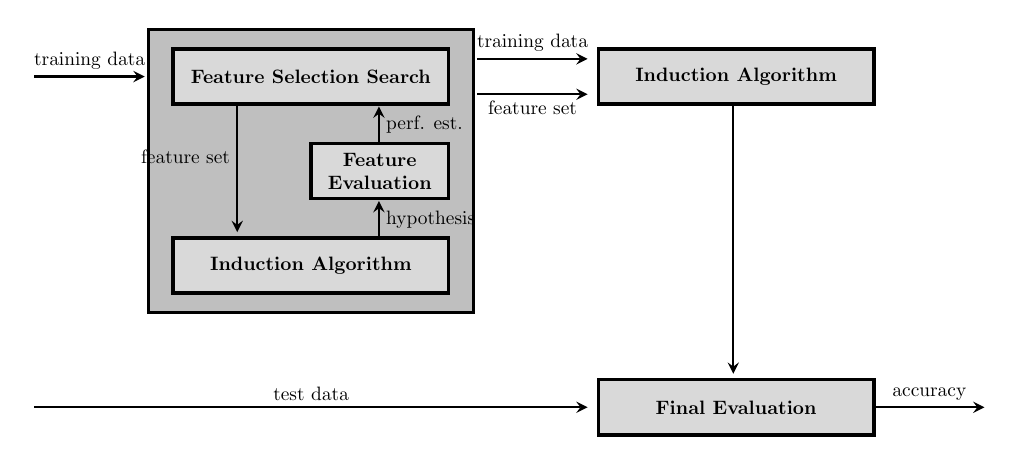
\begin{tikzpicture}[
		scale=0.3,
		every node/.append style={scale=0.7},
		box/.style={draw=black,very thick,minimum width=5cm,minimum height=1cm,align=center,fill=lightgray!60,anchor=east},
		arr/.style={thick,-stealth,shorten >= 0.5mm,shorten <= 0.5mm},
	]

		% wrapper
		\draw[draw=black,very thick,fill=lightgray] (-12.75,-10) rectangle (1,2);
		\draw[arr] (-17.75,0) -- node[above] {training data} ++(5,0);
		
		\draw[arr] (-9,0) -- node[left] {feature set} ++(0,-6.75);
		\draw[arr] (-3,-7) -- node[right] {hypothesis} ++(0,1.9);
		\draw[arr] (-3,-3) -- node[right] {perf. est.} ++(0,1.9);
		
		\node[box] (A) at (0,0) {\textbf{Feature Selection Search}};
		\node[box,minimum width=2.5cm] (B) at (0,-4) {\textbf{Feature} \\ \textbf{Evaluation}};
		\node[box] (C) at (0,-8) {\textbf{Induction Algorithm}};


		% induction algorithm
		\node[box] at (18,0) {\textbf{Induction Algorithm}};
		\draw[arr] (1,0.75) -- node[above] {training data} ++(5,0);
		\draw[arr] (1,-0.75) -- node[below] {feature set} ++(5,0);

		% final evaluation
		\node[box] at (18,-14) {\textbf{Final Evaluation}};
		\draw[arr] (12,-1) -- ++(0,-11.75);
		\draw[arr] (-17.75,-14) -- node[above] {test data} ++(23.75,0);

		\draw[arr] (17.8,-14) -- node[above] {accuracy} ++(5,0);
		
	\end{tikzpicture}
\end{figure}